\section{Thực nghiệm và đánh giá}
\label{sec:benchmark}
\subsection{Câu hỏi thực nghiệm và phạm vi}
Thực nghiệm trước hết kiểm tra hai phiên bản Eclat bằng kết quả
tham chiếu từ SPMF. Sau đó, nhóm khảo sát thời gian chạy, đỉnh bộ nhớ
và ảnh hưởng của số lượng cũng như độ dài giao dịch. So sánh hiệu năng
dựa trên các lượt chạy hoàn tất và trả về kết quả đã đối chiếu.

\subsection{Dữ liệu và ngưỡng hỗ trợ}
Bốn bộ dữ liệu từ FIMI~\cite{fimi} có đặc điểm khác nhau
(Bảng~\ref{tab:data}). Chess và Mushroom có giao dịch dài. Retail
có nhiều mục nhưng mỗi giao dịch thường ngắn. T10I4D100K là dữ liệu
tổng hợp. Số tập phổ biến phụ thuộc vào mức độ đồng xuất hiện của
các mục và ngưỡng hỗ trợ, ngoài quy mô của bộ dữ liệu.

\begin{reporttable}
\caption{Số giao dịch $N$, số mục phân biệt $M$ và độ dài giao dịch trung bình $\bar L$ sau chuẩn hóa.}
\label{tab:data}
\small
\begin{tabular}{lrrr}\toprule
Bộ dữ liệu & $N$ & $M$ & $\bar L$\\\midrule
Chess & 3.196 & 75 & 37,0000\\
Mushroom & 8.124 & 119 & 23,0000\\
Retail & 88.162 & 16.470 & 10,3058\\
T10I4D100K & 100.000 & 870 & 10,1023\\\bottomrule
\end{tabular}
\end{reporttable}

Julia và SPMF nhận cùng dữ liệu sau khi chuẩn hóa. Bước này giữ
nguyên các giao dịch trùng và dùng ánh xạ một-một nếu cần đổi mã mục.
Với mỗi bộ dữ liệu, nhóm chọn bảy mức của ngưỡng hỗ trợ tối thiểu
(\textit{minsup}) rồi áp dụng công thức~\eqref{eq:tv1-threshold}.
Các giá trị cụ thể được liệt kê ở Bảng~\ref{tab:grids} trong phụ lục.

\subsection{Môi trường và phương pháp đo}
\label{sec:measurement-method}
Các phép đo chạy trên cùng môi trường Colab CPU (Broadwell, 2 vCPU,
12,67 GiB RAM). Cài đặt Julia dùng phiên bản 1.13.3 và một luồng.
Mỗi cấu hình có năm lượt đo. Các hình báo cáo trung vị và khoảng
nhỏ nhất đến lớn nhất để thể hiện độ biến thiên giữa các lượt.

\textit{Thời gian toàn tiến trình.} Mỗi lượt dùng một tiến trình
mới, tính từ khi khởi động đến khi ghi xong kết quả. Khoảng đo bao
gồm nạp môi trường, biên dịch JIT, đọc dữ liệu, dựng tập định danh
và khai thác. Chuẩn hóa dữ liệu và đối chiếu kết quả được thực hiện
ngoài khoảng đo này.

\textit{Thời gian khai thác sau làm nóng.} Thí nghiệm về quy mô và
độ dài giao dịch đo lời gọi khai thác sau một lượt chạy chuẩn bị
(\textit{warm-up}) với cùng dữ liệu và ngưỡng.

\textit{Đỉnh bộ nhớ thường trú (Peak RSS).} Đây là giá trị lớn nhất
của bộ nhớ thường trú từ lúc tiến trình khởi động đến khi khai thác
xong, trước khi sắp xếp và ghi kết quả. Giá trị này gồm cả môi trường
Julia, lượt chạy chuẩn bị, dữ liệu đầu vào và các cấu trúc khai thác.

\subsection{Đối chiếu tính đúng đắn}
Một lần đối chiếu đạt khi cài đặt của nhóm và SPMF trả về đúng cùng
các tập mục và cùng số giao dịch hỗ trợ cho từng tập. Hai kết quả
có cùng số lượng vẫn có thể khác nhau ở các tập mục cụ thể. Bảng~\ref{tab:correct}
trình bày kết quả đối chiếu trên năm bộ dữ liệu đầy đủ.

\begin{reporttable}
\caption{Kết quả đối chiếu từng tập mục và số hỗ trợ với SPMF.}
\label{tab:correct}
\footnotesize
\begin{tabular}{lrrr}\toprule
Bộ dữ liệu & Ngưỡng (\%) & Số tập SPMF & Khớp\\\midrule
Groceries & 1 & 333 & 100\%\\
Chess & 87,5 & 1.386 & 100\%\\
Mushroom & 70 & 31 & 100\%\\
Retail & 4 & 18 & 100\%\\
T10I4D100K & 1,5 & 237 & 100\%\\\bottomrule
\end{tabular}
\end{reporttable}

\subsection{Thời gian chạy và số tập mục theo ngưỡng}
Nhóm chạy Set, BitVector và SPMF ở bảy ngưỡng trên mỗi bộ dữ liệu.
Bảng~\ref{tab:runtime-colab} tóm tắt kết quả ở ngưỡng thấp nhất
của từng bộ. Hình~\ref{fig:runtime-colab} so sánh xu hướng trên cả dải.

\begin{reporttable}
\caption{Thời gian toàn tiến trình ở ngưỡng thấp nhất (giây). Trung vị của năm lượt trên Colab. BV là BitVector.}
\label{tab:runtime-colab}
\footnotesize
\begin{tabular}{lrrrrr}\toprule
Bộ dữ liệu & $s$ (\%) & Set & BV & SPMF & Số tập\\\midrule
Chess & 80 & 6,365 & 6,286 & 2,156 & 8.227\\
Mushroom & 40 & 3,890 & 5,147 & 1,235 & 565\\
Retail & 0,5 & 4,617 & 5,052 & 2,598 & 580\\
T10I4D100K & 0,5 & 10,855 & 5,422 & 1,774 & 1.073\\\bottomrule
\end{tabular}
\end{reporttable}

\begin{figure*}[!tbp]
\centering
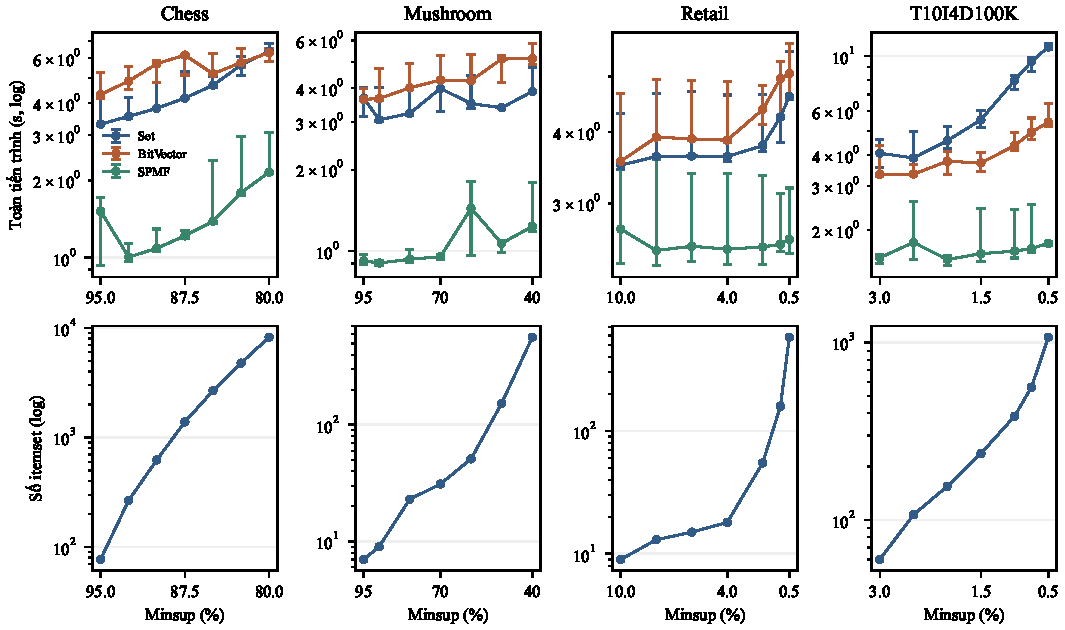
\includegraphics[width=0.90\textwidth]{runtime_counts.pdf}
\caption{Thời gian toàn tiến trình (hàng trên) và số tập phổ biến (hàng dưới) trên bốn bộ dữ liệu theo ngưỡng hỗ trợ giảm dần. Điểm biểu thị trung vị, thanh biểu thị khoảng nhỏ nhất đến lớn nhất. Trục tung dùng thang logarit.}
\label{fig:runtime-colab}
\end{figure*}



SPMF có thời gian toàn tiến trình thấp nhất theo trung vị ở cả
28 cấu hình. Trong hai phiên bản của nhóm, BitVector nhanh hơn
trên T10I4D100K, còn Set nhanh hơn trên Retail ở cả bảy ngưỡng.
Retail có trung bình khoảng 10 mục mỗi giao dịch trên tổng số hơn
16 nghìn mục, nên cách biểu diễn chỉ lưu các định danh xuất hiện
có thể có lợi. Trên Chess ở ngưỡng 80\%, hai
phiên bản chỉ chênh khoảng 1,2\% và khoảng thời gian quan sát
được chồng lấn.

Khi hạ ngưỡng, các tập đã phổ biến được giữ lại và các tập có
số hỗ trợ thấp hơn có thể được bổ sung. Chess có ít giao dịch
nhất nhưng cho nhiều kết quả nhất ở cuối dải khảo sát. Các bộ
dữ liệu dùng các dải ngưỡng khác nhau, nên kết quả này mô tả
xu hướng trong từng dải đã chọn.

\subsubsection{Đối chiếu hiệu năng với SPMF}
Ở ngưỡng thấp nhất của T10I4D100K, thời gian toàn tiến trình của Set
và BitVector lần lượt gấp khoảng 6,12 và 3,06 lần SPMF
(Bảng~\ref{tab:runtime-colab}). Thay biểu diễn Set bằng vector bit
thu hẹp chênh lệch trong cấu hình này, nhưng SPMF vẫn có lợi thế
về thời gian hoàn tất. Trên Mushroom và Retail ở cuối dải ngưỡng,
Set lại gần thời gian của SPMF hơn BitVector. Kết quả vì vậy chưa
ủng hộ việc dùng một biểu diễn duy nhất cho mọi bộ dữ liệu.

Phép đo toàn tiến trình ở Mục~\ref{sec:measurement-method} phản ánh
chi phí của một lượt chạy độc lập. Julia phải nạp môi trường và
biên dịch các lời gọi chưa được thực thi; SPMF cũng chịu chi phí
khởi động JVM, đọc ghi và thực thi Java. Do chưa đo tách công đoạn
hoặc đo khai thác sau làm nóng của SPMF, chưa thể quy chênh lệch
cho riêng ngôn ngữ, phép giao TID-set hay tối ưu nội bộ của SPMF.
So sánh Peak RSS
chỉ gồm Set và BitVector, nên chưa cho phép đối chiếu RAM với SPMF.

\subsection{Đỉnh bộ nhớ ở ngưỡng giữa dải}
Nhóm dùng ngưỡng thứ tư của mỗi bộ dữ liệu. Mỗi lượt đo chạy một
phiên bản trong tiến trình riêng. Bảng~\ref{tab:ram-colab} và
Hình~\ref{fig:ram-colab} tổng hợp trung vị của năm lượt.

\begin{reporttable}
\caption{Peak RSS trung vị (MiB), năm tiến trình cho mỗi phiên bản. $\Delta_M$ là mức giảm từ trung vị của Set sang BV.}
\label{tab:ram-colab}
\small
\begin{tabular}{lrrr}\toprule
Bộ dữ liệu & Set & BV & $\Delta_M$ (\%)\\\midrule
Chess & 385,27 & 374,90 & 2,69\\
Mushroom & 374,90 & 374,90 & 0,00\\
Retail & 444,45 & 378,34 & 14,87\\
T10I4D100K & 437,32 & 418,77 & 4,24\\\bottomrule
\end{tabular}
\end{reporttable}

\begin{figure}[!tbp]
\centering
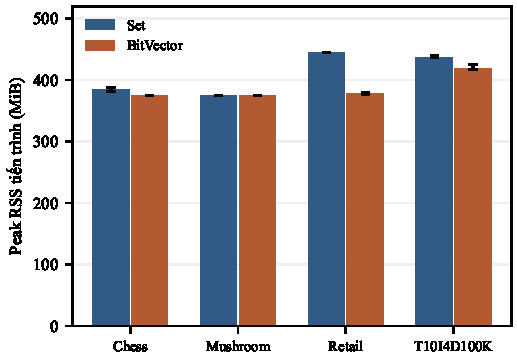
\includegraphics[width=\columnwidth]{peak_ram.pdf}
\caption{Đỉnh bộ nhớ ở ngưỡng giữa dải. Cột biểu thị trung vị và thanh dọc biểu thị khoảng nhỏ nhất đến lớn nhất. Đỉnh gồm cả môi trường Julia và dữ liệu đầu vào.}
\label{fig:ram-colab}
\end{figure}

BitVector có đỉnh bộ nhớ trung vị thấp hơn trên ba bộ dữ liệu,
với mức giảm rõ nhất trên Retail (14,87\%). Với Retail, 7 trên
16.470 mục đạt ngưỡng 4\%, nên việc cấp vector sau khi lọc đặc
biệt có ích. Trên Mushroom, hai trung vị bằng nhau. Đây là mức dùng
bộ nhớ của cả tiến trình theo phạm vi ở Mục~\ref{sec:measurement-method}.

\subsection{Khả năng mở rộng theo số giao dịch}
Nhóm tạo năm tập con lồng nhau từ Retail ở các mức 10\%, 25\%,
50\%, 75\% và 100\%. Ngưỡng hỗ trợ giữ ở 4\%, nên số giao dịch
tối thiểu thay đổi theo kích thước mỗi tập con. Bảng~\ref{tab:scale-colab}
và Hình~\ref{fig:scale-colab} trình bày thời gian khai thác sau làm nóng.

\begin{reporttable}
\caption{Khả năng mở rộng trên Retail: trung vị thời gian khai thác sau làm nóng (ms), năm lượt/cấu hình.}
\label{tab:scale-colab}
\footnotesize
\begin{tabular}{rrrrr}\toprule
Tỷ lệ (\%) & $N$ & $c_{\min}$ & Set & BV\\\midrule
10 & 8.816 & 353 & 25,08 & 6,10\\
25 & 22.040 & 882 & 68,92 & 16,71\\
50 & 44.081 & 1.764 & 158,70 & 33,80\\
75 & 66.121 & 2.645 & 276,07 & 49,34\\
100 & 88.162 & 3.527 & 358,41 & 62,95\\\bottomrule
\end{tabular}
\end{reporttable}

\begin{figure}[!tbp]
\centering
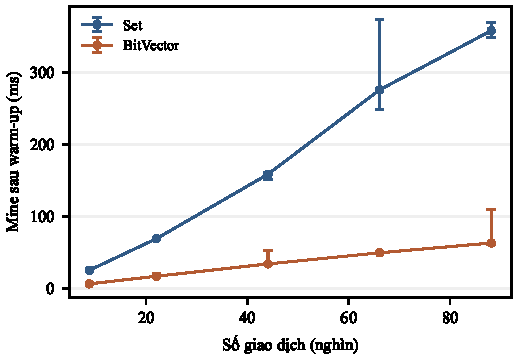
\includegraphics[width=\columnwidth]{scalability.pdf}
\caption{Khả năng mở rộng trên năm tập con lồng nhau của Retail. Điểm biểu thị trung vị và thanh biểu thị khoảng nhỏ nhất đến lớn nhất. Hai phiên bản khớp SPMF ở mọi mức.}
\label{fig:scale-colab}
\end{figure}

Hình~\ref{fig:scale-colab} cho thấy khi $N$ tăng khoảng mười lần,
trung vị của Set tăng 14,29 lần, còn BitVector tăng 10,32 lần. Cả năm mức đều
có 18 tập mục, nên số kết quả giữ nguyên trong thí nghiệm này. BitVector
có xu hướng tăng gần tỷ lệ với $N$ trong miền đã đo. Thời gian của Set tăng nhanh hơn.
Xu hướng này chỉ mô tả các tập con Retail và ngưỡng đã khảo sát.

\subsection{Phân tích đánh đổi giữa thời gian và bộ nhớ}
Trên Retail tại ngưỡng hỗ trợ 4\%, BitVector có Peak RSS trung vị
378,34 MiB, giảm 14,87\% so với mức 444,45 MiB của Set.
Thời gian toàn tiến trình của BitVector là 3,869 giây, cao hơn
mức 3,624 giây của Set, theo số đo đầy đủ của Hình~\ref{fig:runtime-colab}.
Trong thí nghiệm mở rộng theo số giao dịch,
trên toàn bộ 88.162 giao dịch và cùng ngưỡng hỗ trợ, thời gian
khai thác sau làm nóng lần lượt là 62,95 ms và 358,41 ms.

Sự khác biệt trong cách dựng biểu diễn dọc giúp giải thích xu hướng
bộ nhớ. Phiên bản Set dựng tập định danh giao dịch cho toàn bộ
16.470 mục rồi mới lọc các mục không đạt ngưỡng. Phiên bản BitVector
đếm số hỗ trợ trước và chỉ cấp vector cho 7 mục đạt ngưỡng 4\%.
Với $N$ giao dịch và $F_1$ mục đạt ngưỡng, các vector ban đầu cần
$O(F_1N)$ bit, bên cạnh trạng thái đếm $O(M)$ cho $M$ mục phân biệt.
Lọc trước cấp phát giảm số cấu trúc phải dựng khi có nhiều mục hiếm.
Do Peak RSS đo toàn tiến trình và hai phiên bản đồng thời thay đổi
cấu trúc lưu trữ lẫn quy trình cấp phát, chưa thể tách đóng góp
của từng yếu tố vào mức giảm bộ nhớ.

Phép đo sau làm nóng bao gồm cả dựng biểu diễn dọc và duyệt các nhánh
Eclat. Trên Retail ở ngưỡng đang xét, kết quả chỉ có 18 tập phổ biến.
Chênh lệch thời gian vì vậy cần được xem xét cùng chi phí lọc trước
cấp phát đã nêu ở trên. Các phép giao theo từ máy
cũng có thể đóng góp vào lợi thế của BitVector, nhưng chưa đủ cơ sở
quy toàn bộ chênh lệch cho thao tác này khi hai công đoạn chưa được đo riêng.

Hai phiên bản dùng chung mã đọc ghi và trả về cùng kết quả. Tuy vậy,
chưa có số đo từng công đoạn để giải thích chênh lệch 0,245 giây của
thời gian toàn tiến trình. Chỉ số này phù hợp với lượt chạy độc lập;
thời gian sau làm nóng phù hợp với khai thác khi mã đã được biên dịch.
Lựa chọn phiên bản cần xét cả bối cảnh chạy và giới hạn RAM.

\subsection{Ảnh hưởng của độ dài giao dịch}
Nhóm tạo 5.000 giao dịch từ 64 mục và tăng độ dài mỗi giao dịch
từ 4 lên 20, với năm mức khảo sát. Số giao dịch, số mục có thể
chọn và ngưỡng hỗ trợ 5\% được giữ cố định. Bảng~\ref{tab:length-colab}
và Hình~\ref{fig:length-colab} cho thấy thời gian cùng số tập phổ
biến ở từng mức.

\begin{reporttable}
\caption{Dữ liệu tổng hợp và trung vị thời gian khai thác sau làm nóng (ms), qua năm lượt mỗi cấu hình.}
\label{tab:length-colab}
\footnotesize
\begin{tabular}{rrrrr}\toprule
$L$ & Mật độ (\%) & Số tập & Set & BV\\\midrule
4 & 6,25 & 64 & 23,81 & 1,40\\
8 & 12,50 & 64 & 51,29 & 2,39\\
12 & 18,75 & 64 & 85,16 & 3,14\\
16 & 25,00 & 2.077 & 691,57 & 10,18\\
20 & 31,25 & 2.080 & 1.055,70 & 11,10\\\bottomrule
\end{tabular}
\end{reporttable}

\begin{figure*}[!tbp]
\centering
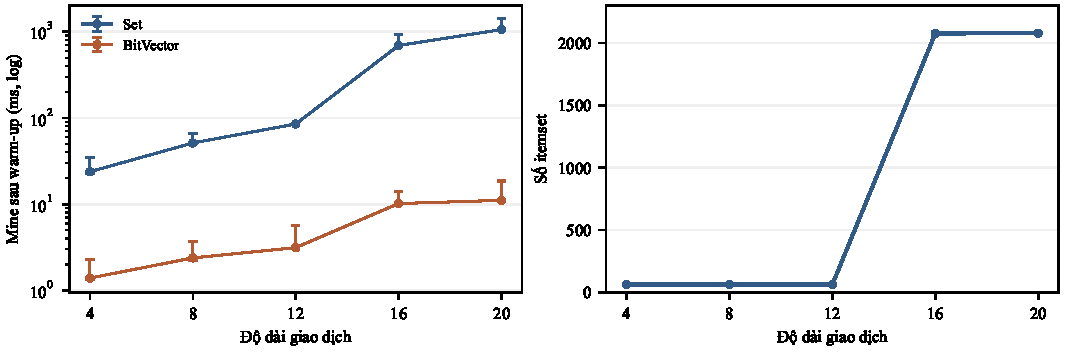
\includegraphics[width=\textwidth]{transaction_length.pdf}
\caption{Ảnh hưởng độ dài giỏ với $N=5.000$, $M=64$, ngưỡng hỗ trợ cố định ở 5\%. Trái: trung vị và khoảng biến thiên của thời gian khai thác trên trục tung log. Phải: số tập mục khớp SPMF ở cả hai phiên bản.}
\label{fig:length-colab}
\end{figure*}

Bước tăng từ 12 lên 16 mục mỗi giao dịch làm số kết quả tăng từ
64 lên 2.077. Giỏ dài hơn làm tăng khả năng hai mục xuất hiện cùng
nhau, nên nhiều cặp vượt ngưỡng 250 giao dịch. Eclat vì thế giữ thêm
các nhánh mở rộng và thực hiện nhiều công việc hơn. Khi độ dài tăng
tiếp lên 20 mục, số kết quả gần như giữ nguyên nhưng thời gian của
Set vẫn tăng đáng kể. Số tập được trả về vì vậy chỉ giải thích một
phần chi phí khai thác.

Với $N$ giữ cố định, chi phí quét một vector bit cho mỗi phép giao
vẫn tỷ lệ với $\lceil N/w\rceil$, trong đó $w$ là số bit mỗi từ máy.
Ở Set, chi phí giao kỳ vọng tỷ lệ với tập định danh nhỏ hơn; khi
giỏ dài lên, nhiều mục có mặt trong nhiều giao dịch hơn, làm tăng
khối lượng định danh cần xử lý. Cơ chế này phù hợp với việc thời gian
Set tiếp tục tăng khi $L$ từ 16 lên 20 dù số kết quả gần như không đổi.
Tuy nhiên, thực nghiệm chưa ghi số ứng viên và kích thước từng tập
định danh, nên chưa xác định riêng phần thời gian tăng do giao tập,
dựng biểu diễn hay cấp phát tạm.

\subsection{Thảo luận và giới hạn thực nghiệm}
Cả 560 lượt đo đều hoàn tất và cho kết quả khớp với SPMF. Lợi thế về
thời gian của mỗi phiên bản phụ thuộc vào độ thưa của tập định danh,
dải ngưỡng và phạm vi đo. Xu hướng quan sát được trên một môi trường
Colab, với năm lượt cho mỗi cấu hình, cần được kiểm tra trên các môi
trường và bộ dữ liệu khác trước khi khái quát.

Có hai hướng tối ưu tiếp theo. Thứ nhất, có thể chọn cấu trúc thưa
hay vector bit theo mật độ của từng tập định danh và đo cả chi phí
chuyển đổi. Thứ hai, có thể dùng lại bộ đệm trong quá trình duyệt
theo chiều sâu để giảm cấp phát khi tính giao. Thí nghiệm tách
riêng từng thay đổi sẽ cho biết phần đóng góp của mỗi kỹ thuật.
